% =============================================================================
% Appendix
% =============================================================================

\section{System Algorithms}
\label{app:algorithms}

This appendix provides complete pseudocode for the two core algorithmic loops that drive \textsc{DeepTutor}: the closed-loop personalized tutoring cycle~(\S\ref{app:algorithm}) and the TutorBot autonomous agent loop~(\S\ref{app:tutorbot}).

\subsection{Closed-Loop Tutoring}
\label{app:algorithm}

Algorithm~\ref{alg:loop} provides the complete pseudocode for the closed-loop personalized tutoring cycle described in \S\ref{sec:cycle}.
At the start of each session, the personalization engine injects the current learner profile and relevant traces into the working context.
Depending on the task type, the pipeline dispatches to either the three-stage problem-solving path (Stages~\ding{172}--\ding{174}) or the two-stage question-generation path (Stages~\ding{175}--\ding{176}).
After every interaction, the resulting trace is appended to the forest and the three memory agents update the learner profile in parallel.

\begin{algorithm}[ht!]
\caption{Closed-Loop Personalized Tutoring}\label{alg:loop}
\small
\begin{algorithmic}[1]
\Require learner profile $\mathcal{D}^{(0)}$;\; trace forest $\mathcal{F}^{(0)} = \emptyset$
\For{session $j = 1, 2, \ldots$}
    \State $\mathcal{C}_{\text{mem}} \gets \Call{ProfileInject}{\mathcal{D}^{(j{-}1)}, \mathcal{F}^{(j{-}1)}, \text{task}_j}$
    \If{$\text{task}_j = (\textsc{Solve},\, q)$}
        \State $\mathcal{C}_{\text{rag}} \gets \textsc{RagTool}(q)$
        \State $\mathcal{E}_{\text{plan}} \gets \Call{Investigate}{q,\;\mathcal{C}_{\text{rag}},\;\mathcal{C}_{\text{mem}},\;\mathcal{F}^{(j{-}1)}}$ \Comment{\ding{172}}
        \State $\mathcal{P}{=}\langle s_1,\dots,s_K\rangle \gets \Call{Plan}{q,\;\mathcal{E}_{\text{plan}},\;\mathcal{C}_{\text{mem}}}$
        \For{$k = 1$ \textbf{to} $K$} \Comment{\ding{173}}
            \While{$s_k$ not resolved}
                \State $(\alpha_t,\, \mathbf{s}_t) \gets \Call{ToolAgent}{q, \mathcal{P}, \mathcal{S}, \mathcal{C}_{\text{rag}}, \mathcal{C}_{\text{mem}}}$
                \State $\mathcal{S} \gets \mathcal{S} \cup \{\mathbf{s}_t\}$
                \If{$\alpha_t = \textsc{Replan}$}
                    \State $\mathcal{P} \gets \Call{Revise}{\mathcal{P}, \mathcal{S}}$
                \EndIf
            \EndWhile
            \State $\mathcal{S} \gets \Call{Compress}{\mathcal{S}, k}$
        \EndFor
        \State $a \gets \Call{IterativeWrite}{\mathcal{S},\;\mathcal{C}_{\text{mem}}}$ \Comment{\ding{174}}
        \State $T_j \gets \Call{BuildTrace}{q, a}$
    \Else \Comment{$\text{task}_j = (\textsc{Generate},\, \tau)$}
      \State $\mathcal{C}_{\text{rag}} \gets \textsc{RagTool}(\tau)$
        \State $f_{\text{idea}} \gets \emptyset$
        \Repeat
            \State $\mathcal{I} \gets \Call{IdeaAgent}{\tau,\;\mathcal{C}_{\text{rag}},\;\mathcal{C}_{\text{mem}},\;f_{\text{idea}}}$ \Comment{\ding{175}}
            \State $(\textit{continue},\, f_{\text{idea}},\, \mathcal{T}_{1..N}) \gets \Call{EvaluateIdeas}{\mathcal{I},\;\tau,\;\mathcal{C}_{\text{mem}}}$
        \Until{$\lnot\,\textit{continue}$}
        \For{$i = 1$ \textbf{to} $N$} \Comment{\ding{176}}
            \Repeat
                \State $(q_i, a_i) \gets \Call{Generator}{\mathcal{T}_i,\;\mathcal{C}_{\text{rag}},\;\mathcal{C}_{\text{mem}}}$
                \State $(\textit{pass}, f_i) \gets \Call{Validator}{q_i, a_i, \mathcal{T}_i}$
                \If{$\lnot\,\textit{pass}$} $\mathcal{T}_i \gets \Call{Revise}{\mathcal{T}_i, f_i}$
                \EndIf
            \Until{\textit{pass}}
        \EndFor
        \State $T_j \gets \Call{BuildTrace}{\tau, \{(q_i, a_i)\}}$
    \EndIf
    \State $\mathcal{F}^{(j)} \gets \mathcal{F}^{(j{-}1)} \cup \{T_j\}$
    \State $\mathcal{D}^{(j)} \gets \Call{MemoryUpdate}{\mathcal{D}^{(j{-}1)}, T_j}$
\EndFor
\end{algorithmic}
\end{algorithm}

% ============================================================
\subsection{TutorBot Autonomous Agent Loop}
\label{app:tutorbot}
% ============================================================

Algorithm~\ref{alg:tutorbot} provides the pseudocode for the TutorBot autonomous agent loop described in \S\ref{sec:agentloop}.
Each inbound message triggers a three-phase cycle: context assembly, iterative tool-augmented reasoning, and memory consolidation.
The \textsc{BuildContext} procedure weaves the bot's persona (Soul), long-term memory, skill descriptions, and conversation history into a single prompt.
The inner ReAct loop calls the LLM, executes any requested tools, and appends results until a final response is produced or the iteration budget is exhausted.
After each turn, the memory consolidator checks whether the accumulated history exceeds half the context window; if so, it distills the oldest unconsolidated messages into the two-layer persistent memory (long-term profile and session history log), advancing the consolidation pointer to reclaim context space for future turns.

\begin{algorithm}[ht!]
\caption{TutorBot Autonomous Agent Loop}\label{alg:tutorbot}
\small
\begin{algorithmic}[1]
\Require message bus $\mathcal{B}$;\; LLM provider $\mathcal{M}$;\; tool registry $\mathcal{T}$;\; session store $\mathcal{S}$;\; context window $W$;\; max iterations $I_{\max}$
\Statex
\Loop \Comment{Main event loop}
    \State $m \gets \mathcal{B}.\textsc{ConsumeInbound}()$ \Comment{Block until next message}
    \State $\sigma \gets \mathcal{S}.\textsc{GetOrCreate}(m.\textit{session\_key})$
    \Statex
    \Comment{\textbf{Phase 1: Context Assembly}}
    \State $\textit{sys} \gets \textsc{BuildContext}(\sigma.\textit{soul},\; \sigma.\textit{memory},\; \sigma.\textit{skills})$
    \State $H \gets \sigma.\textsc{GetHistory}()$ \Comment{Unconsolidated messages}
    \State $\textit{msgs} \gets [\textit{sys}] \,\|\, H \,\|\, [\textsc{Wrap}(m)]$
    \Statex
    \Comment{\textbf{Phase 2: ReAct Tool-Calling Loop}}
    \For{$i = 1$ \textbf{to} $I_{\max}$}
        \State $r \gets \mathcal{M}.\textsc{Chat}(\textit{msgs},\; \mathcal{T}.\textsc{Definitions}())$
        \If{$r$ has no tool calls}
            \State $\textit{response} \gets r.\textit{content}$ \Comment{Final answer}
            \State \textbf{break}
        \EndIf
        \State Append assistant message (with tool calls) to $\textit{msgs}$
        \ForAll{tool call $\tau$ in $r.\textit{tool\_calls}$}
            \State $\textit{result} \gets \mathcal{T}.\textsc{Execute}(\tau.\textit{name},\; \tau.\textit{args})$
            \State Append tool result to $\textit{msgs}$
        \EndFor
    \EndFor
    \Statex
    \Comment{\textbf{Phase 3: Persist \& Consolidate}}
    \State $\sigma.\textsc{AppendTurn}(\textit{msgs})$
    \If{$\textsc{EstimateTokens}(\sigma) > W$} \Comment{Context pressure}
        \State $\textit{chunk} \gets \sigma.\textit{messages}[\sigma.\textit{ptr} : \textit{boundary}]$
        \State $\textsc{Consolidate}(\textit{chunk},\; \sigma.\textit{memory})$ \Comment{LLM-based distillation}
        \State $\sigma.\textit{ptr} \gets \textit{boundary}$
    \EndIf
    \State $\mathcal{S}.\textsc{Save}(\sigma)$
    \State $\mathcal{B}.\textsc{PublishOutbound}(\textit{response},\; m.\textit{channel})$
\EndLoop
\end{algorithmic}
\end{algorithm}

The \textsc{BuildContext} procedure constructs the system prompt by concatenating the following components in order:
(1)~the bot's core identity and runtime metadata,
(2)~bootstrap files including the Soul template (persona), user preferences, and tool guidelines,
(3)~long-term memory (user profile and learning context summaries),
(4)~always-active skill descriptions, and
(5)~a summary of all available skills for on-demand loading.
The \textsc{Consolidate} procedure invokes the LLM with a dedicated ``memory consolidation agent'' system prompt, forcing a structured tool call that produces both a timestamped history entry (appended to the session log) and an updated long-term profile (overwriting the previous version).
This two-output design ensures that consolidation simultaneously preserves searchable event detail and maintains a concise, current learner model.

% ============================================================
\section{Extended Evaluation Details}
\label{app:eval}
% ============================================================

\subsection{Evaluation Rubrics}
\label{app:eval:rubrics}

Each of the ten metrics is evaluated on a 1--5 Likert scale by an LLM judge.
Below we provide the defining criteria for each metric.

\paragraph{Solve-Side Metrics.}
\begin{itemize}[nosep,leftmargin=*]
\item \textbf{Source Faithfulness~(SF)}: factual consistency with the source material, terminological precision, grounding in retrieved evidence, and explicit source attribution.
\item \textbf{Personalization~(PER)}: tailoring to the specific learner's diagnosed misunderstandings and conversational trajectory.
\item \textbf{Applicability~(APP)}: provision of concrete, immediately actionable guidance.
\item \textbf{Vividness~(VID)}: richness of multimodal delivery elements (examples, analogies, structured formatting) that enhance understanding.
\item \textbf{Logical Depth~(LD)}: presence of explicit, multi-step causal reasoning chains.
\end{itemize}

\paragraph{Practice-Side Metrics.}
\begin{itemize}[nosep,leftmargin=*]
\item \textbf{Fitness~(FIT)}: alignment with session-level diagnosed weaknesses at an appropriate difficulty level.
\item \textbf{Groundedness~(GND)}: factual anchoring in the source material.
\item \textbf{Diversity~(DIV)}: novelty in angle and cognitive demand across generated questions.
\item \textbf{Answer Quality~(ANS)}: correctness of the answer key and plausibility of distractors.
\item \textbf{Cross Concept~(CC)}: meaningful integration of multiple concepts within a single question.
\end{itemize}

\subsection{Student Simulator}
\label{app:eval:simulator}

\begin{figure*}[t]
    \centering
    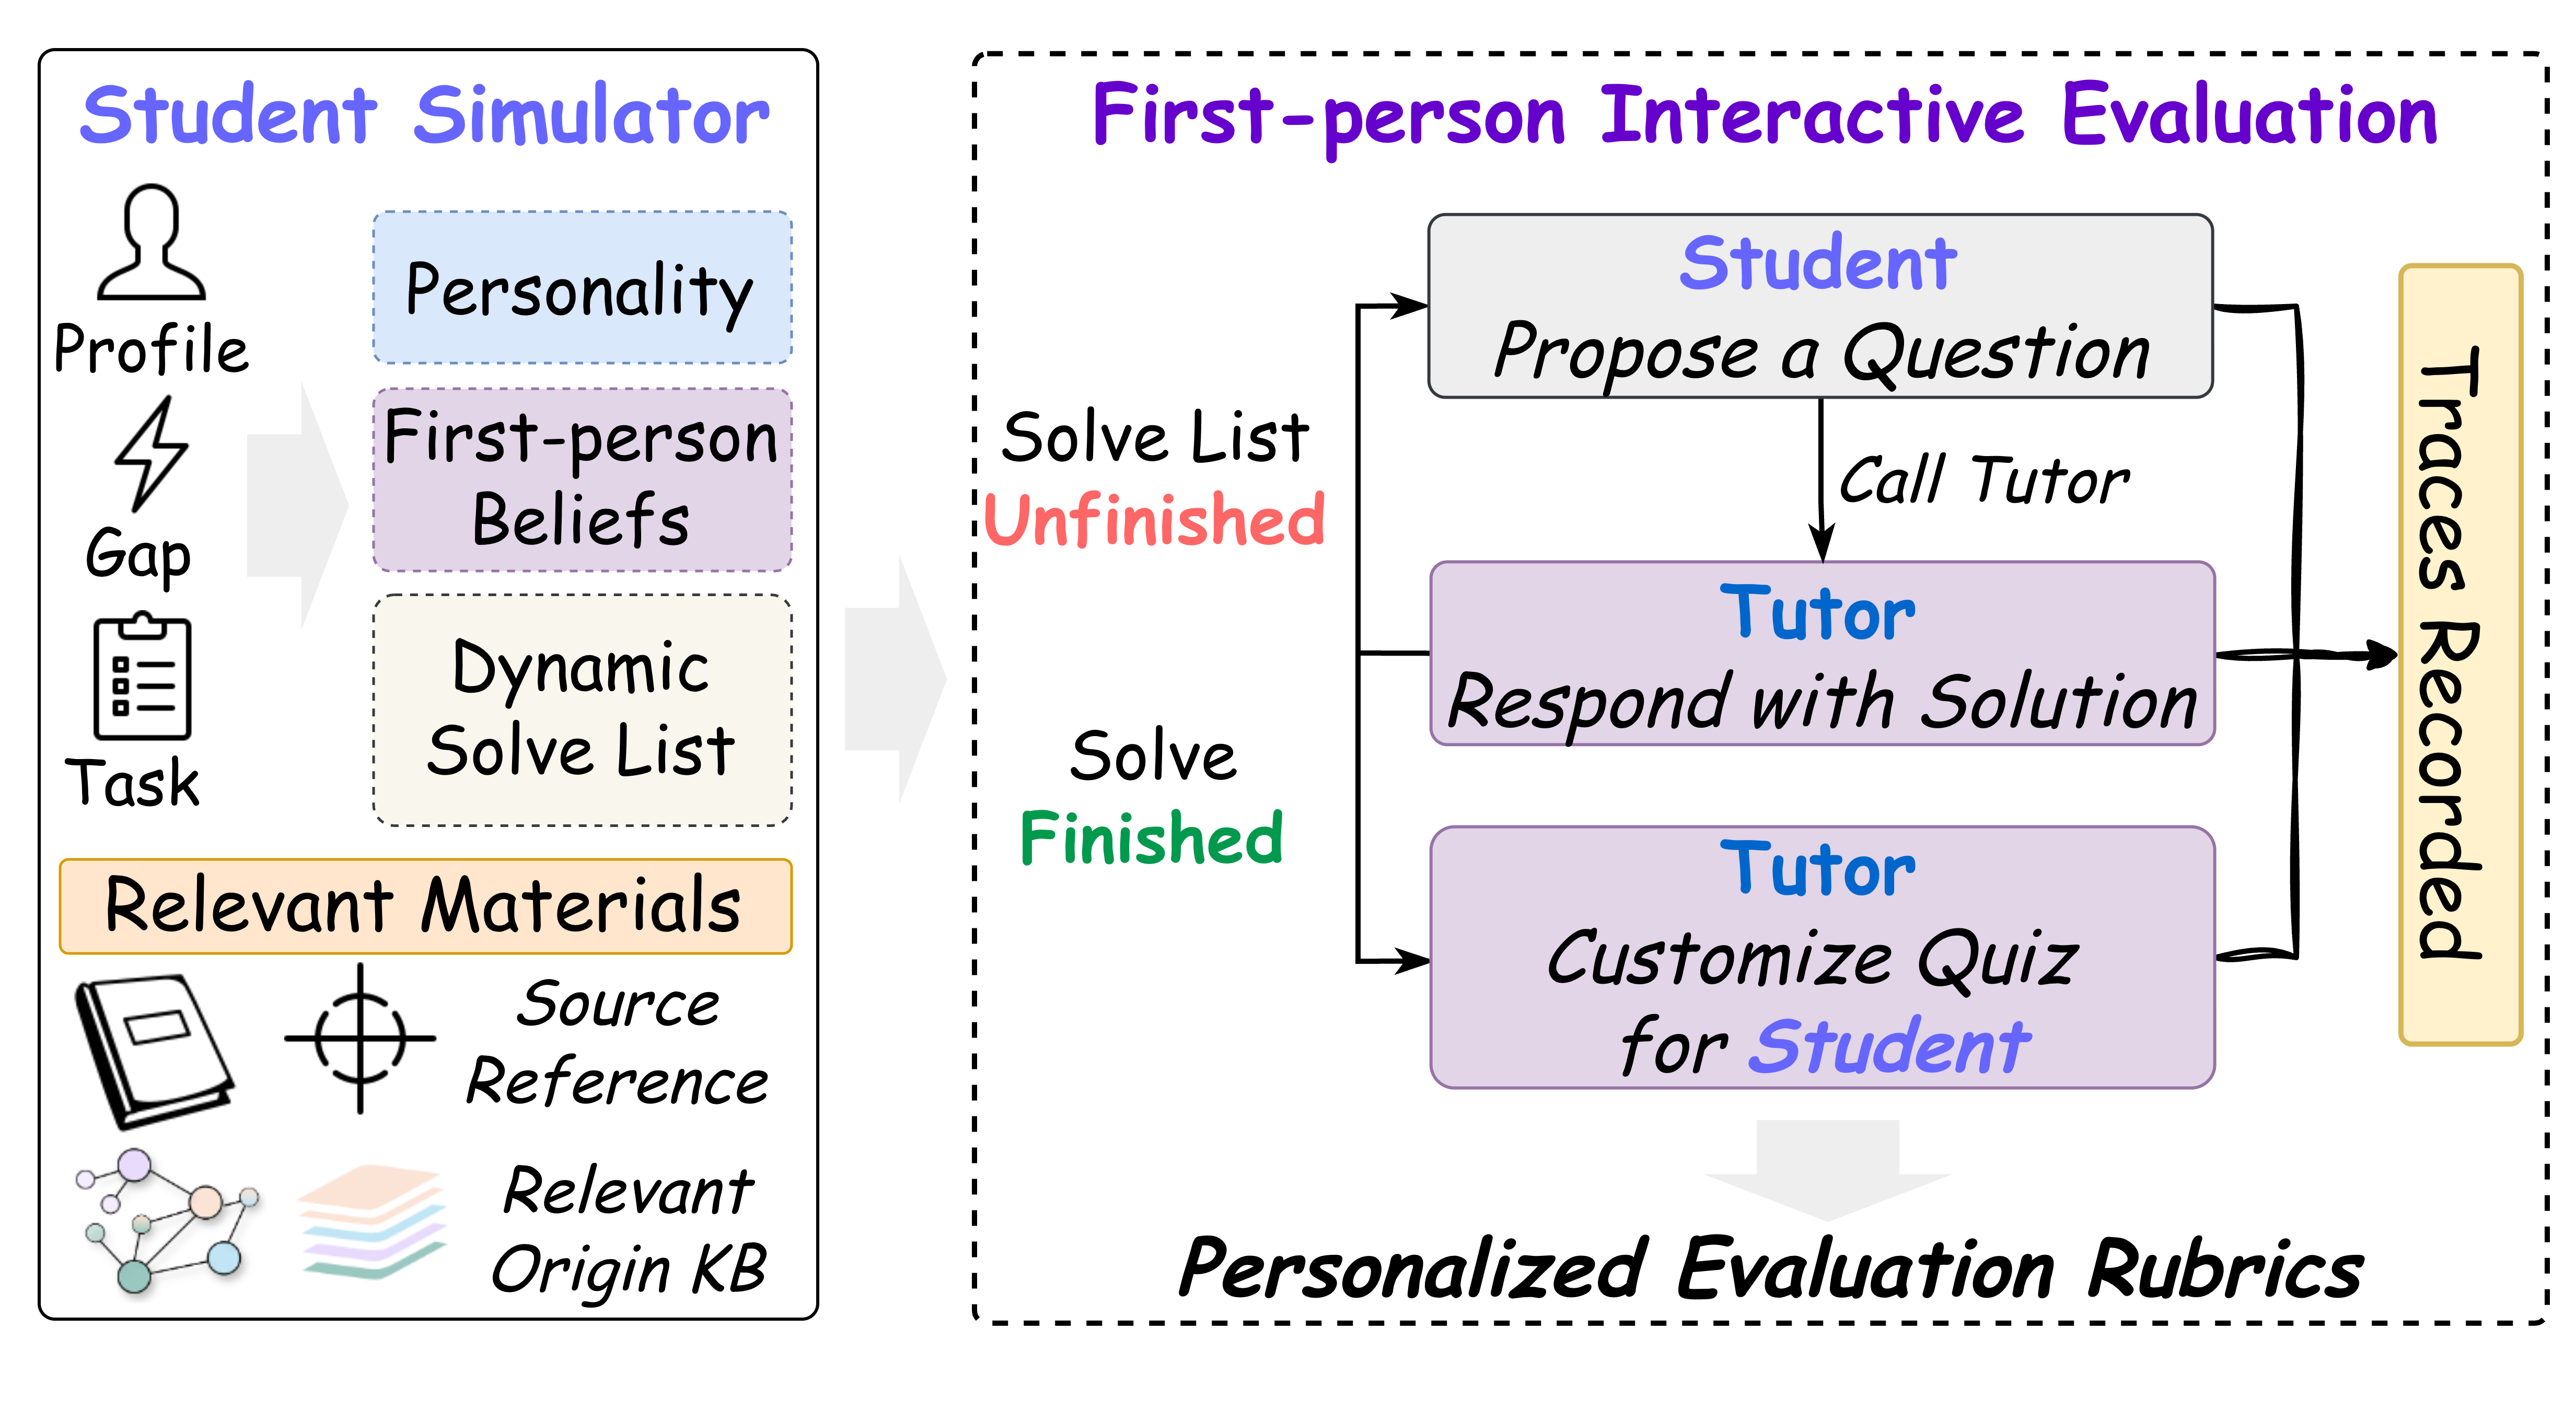
\includegraphics[width=\textwidth]{figures/eval-0315.png}
    \caption{First-person interactive evaluation protocol. A student simulator initialized from a \textsc{TutorBench} entry engages the tutoring system in multi-turn dialogue; the resulting transcript is scored against a personalized rubric by an independent judge.}
    \label{fig:evaluation}
\end{figure*}

The student simulator is an LLM agent initialized from a \textsc{TutorBench} entry comprising a learner profile, knowledge gaps, and an interactive task.
Each gap is pre-transformed into a first-person belief statement so that the simulator \emph{acts as} the student rather than narrating errors from an external perspective.
Listing~\ref{lst:simulator} gives the system prompt governing simulator behavior; template variables are populated from the entry at initialization time.

\begin{lstlisting}[caption={Student Simulator System Prompt},label={lst:simulator}]
You are role-playing as a student seeking help from an AI
tutor. Stay in character throughout the entire conversation.

# Who You Are
{personality}

# Your Background
{education_background}

# Why You Are Here
{learning_purpose}

# What You Know
You are confident about these topics:
{known_well}

You have vague or partial understanding:
{partially_known}

You have NO knowledge of the following:
{unknown}

# What You Believe (IMPORTANT -- these feel true to you)
{beliefs}

# Behavioral Rules
1. NEVER display knowledge listed as "unknown".
2. When the tutor teaches something new, try to rephrase
   it in your own words. It's okay to rephrase imperfectly.
3. If the tutor asks "do you understand?", be honest based
   on whether the explanation addressed your confusion.
4. Keep responses concise: 1-4 sentences typically.
5. Stay consistent with your personality throughout.
6. You may ask follow-up questions or request examples.
7. When you feel you've understood, PREFER asking for a
   practice problem before ending.

# Ending the conversation (ONLY when done)
Use [ACTION: task_complete] ONLY if ALL conditions are true:
- You are explicitly done.
- You have zero remaining questions.
- You are NOT requesting anything else.
- Your message is a natural closing/goodbye.
\end{lstlisting}

\paragraph{Dynamic Gap Pacing.}
The \texttt{\{beliefs\}} placeholder is populated with first-person formulations of each knowledge gap (e.g., ``I think the Poynting vector always points in the direction of wave propagation'').
The simulator's behavioral rules enforce realistic resistance patterns: the student may defend misconceptions, partially accept corrections, and only signal completion after sufficient scaffolded explanation.
This prevents trivially short sessions where the student immediately agrees with any tutor statement.

\subsection{Baseline Definitions}
\label{app:eval:baselines}

All baselines share the same backbone (\emph{Gemini-3-Flash}) and knowledge-base access as \textsc{DeepTutor}.
Each baseline receives the student's question together with the top-$k$ RAG-retrieved passages and a tutoring-oriented system prompt; they differ only in the reasoning strategy applied before producing the final response.

\paragraph{Notation.}
All baseline algorithms share the following primitives:
$\textsc{Rag}(m, K, \textit{mode}, k)$ retrieves $k$~passages from knowledge base~$K$ for query~$m$;
$\textsc{Concat}(\cdot)$ concatenates its arguments into a single context string; and
$\textsc{Llm}(p, H, \textit{ctx})$ denotes one LLM generation call with system prompt~$p$, conversation history~$H$, and user-side context~\textit{ctx}.

\paragraph{Naive Tutor.}
The simplest baseline: a single LLM call maps the concatenation of the system prompt, RAG context, and user question directly to a response.
No intermediate reasoning, self-critique, or tool use is involved.

\begin{algorithm}[ht!]
\caption{Naive Tutor}\label{alg:naive}
\small
\begin{algorithmic}[1]
\Require Student message $m$, history $H$, knowledge base $K$
\Statex \textbf{Prompt:} $p_{\text{tutor}}$ (tutoring persona)
\State $r_{\text{rag}} \gets \textsc{Rag}(m, K, \textit{naive}, k{=}2)$
\State $\textit{ctx} \gets \textsc{Concat}(r_{\text{rag}}, m)$
\State $\textit{response} \gets \textsc{Llm}(p_{\text{tutor}}, H, \textit{ctx})$
\State \Return \textit{response}
\end{algorithmic}
\end{algorithm}

\paragraph{CoT Tutor.}
Identical to the Naive Tutor except that the system prompt appends an explicit chain-of-thought directive~\citep{wei2022chain}, instructing the model to ``think step by step'' before answering.
The reasoning trace and the final answer are produced in one LLM call.

\begin{algorithm}[ht!]
\caption{CoT Tutor}\label{alg:cot}
\small
\begin{algorithmic}[1]
\Require Student message $m$, history $H$, knowledge base $K$
\Statex \textbf{Prompt:} $p_{\text{cot}}$ (tutoring persona + chain-of-thought directive)
\State $r_{\text{rag}} \gets \textsc{Rag}(m, K, \textit{naive}, k{=}2)$
\State $\textit{ctx} \gets \textsc{Concat}(r_{\text{rag}}, m)$
\State $\textit{response} \gets \textsc{Llm}(p_{\text{cot}}, H, \textit{ctx})$
\State \Return \textit{response}
\end{algorithmic}
\end{algorithm}

\paragraph{Self-Refine Tutor.}
A two-pass pipeline inspired by~\citet{madaan2024selfrefine}.
In the first pass, the model generates an initial draft answer.
In the second pass, a pedagogical review prompt asks the same model to critique the draft for factual accuracy, personalization, and clarity, then produce a revised response.

\begin{algorithm}[ht!]
\caption{Self-Refine Tutor}\label{alg:selfrefine}
\small
\begin{algorithmic}[1]
\Require Student message $m$, history $H$, knowledge base $K$
\Statex \textbf{Prompts:} $p_{\text{tutor}}$ (tutoring persona), $p_{\text{ref}}$ (pedagogical reviewer)
\State $r_{\text{rag}} \gets \textsc{Rag}(m, K, \textit{naive}, k{=}2)$
\State $\textit{ctx} \gets \textsc{Concat}(r_{\text{rag}}, m)$
\State $\textit{draft} \gets \textsc{Llm}(p_{\text{tutor}}, H, \textit{ctx})$ \Comment{initial response}
\State $\textit{ctx}' \gets \textsc{Concat}(r_{\text{rag}}, m, \textit{draft})$
\State $\textit{response} \gets \textsc{Llm}(p_{\text{ref}}, H, \textit{ctx}')$ \Comment{refine for clarity \& pedagogy}
\State \Return \textit{response}
\end{algorithmic}
\end{algorithm}

\paragraph{ReAct Tutor.}
A single-round ReAct-inspired loop~\citep{yao2023reactsynergizingreasoningacting} per student turn via four sequential LLM calls: $p_{\text{think}}$ diagnoses the student's need; $p_{\text{act}}$ decides on a tutoring action plan; $p_{\text{obs}}$ reviews the thought--action pair; and $p_{\text{tutor}}$ synthesizes the accumulated reasoning into a final response.
Relative to \textsc{DeepTutor}, this baseline does not include a multi-step planner, external tool execution beyond the shared naive RAG context, or cross-session memory.

\begin{algorithm}[ht!]
\caption{ReAct Tutor (single-round per turn)}\label{alg:react}
\small
\begin{algorithmic}[1]
\Require Student message $m$, history $H$, knowledge base $K$
\Statex \textbf{Prompts:} $p_{\text{think}},\; p_{\text{act}},\; p_{\text{obs}},\; p_{\text{tutor}}$
\State $r \gets \textsc{Rag}(m, K, \textit{naive}, k{=}2)$
\State $c_0 \gets \textsc{Concat}(r, H, m)$ \Comment{base context}
\State $\textit{th} \gets \textsc{Llm}(p_{\text{think}}, c_0)$ \Comment{diagnose need}
\State $\textit{act} \gets \textsc{Llm}(p_{\text{act}}, \textsc{Concat}(c_0, \textit{th}))$ \Comment{plan action}
\State $\textit{obs} \gets \textsc{Llm}(p_{\text{obs}}, \textsc{Concat}(c_0, \textit{th}, \textit{act}))$ \Comment{review}
\State $\textit{resp} \gets \textsc{Llm}(p_{\text{tutor}}, H, \textsc{Concat}(c_0, \textit{th}, \textit{act}, \textit{obs}))$
\State \Return \textit{resp}
\end{algorithmic}
\end{algorithm}

\subsection{General Problem-Solving Setup}
\label{app:eval:general}

Tables~\ref{tab:benchmarks} and~\ref{tab:backbones} summarize the benchmarks and backbone models used for the general problem-solving evaluation reported in \S\ref{sec:generalization}.
Note that several benchmarks are evaluated on subsets rather than the full release: HLE uses a fixed 500-question subset, LiveBench uses only the reasoning subset, and GAIA scores are reported per difficulty level (L1--L3).

\begin{table}[ht!]
\centering
\small
\begin{tabular}{@{}llcc@{}}
\toprule
\textbf{Benchmark} & \textbf{Category} & \textbf{Size} & \textbf{Format} \\
\midrule
HLE~\citep{phan2025hle} & STEM reasoning & 500$^\dagger$ & open-ended \\
GPQA-Diamond~\citep{rein2024gpqa} & STEM reasoning & 198 & 4-choice MCQ \\
LiveBench~\citep{white2025livebench} & reasoning & subset$^\dagger$ & mixed \\
GAIA~\citep{mialon2024gaia} & agentic & 165 & open-ended \\
AA-LCR~\citep{artificialanalysis2025lcr} & long-context & 100 & open-ended \\
\bottomrule
\end{tabular}
\caption{Public benchmarks used in the general problem-solving evaluation.
$^\dagger$HLE uses a fixed 500-question subset; LiveBench uses the reasoning subset only.}
\label{tab:benchmarks}
\end{table}

All five backbone models are accessed via API.
Qwen-3.5-Plus is called through Alibaba Cloud (DashScope); the remaining four models are called through OpenRouter.
Table~\ref{tab:backbones} lists the exact model identifiers used.

\begin{table}[ht!]
\centering
\small
\begin{tabular}{@{}llll@{}}
\toprule
\textbf{Backbone} & \textbf{API Source} & \textbf{Model Name} & \textbf{Context} \\
\midrule
Gemini-3-Flash  & OpenRouter    & \texttt{google/gemini-3-flash}       & 1M \\
Sonnet-4.5      & OpenRouter    & \texttt{anthropic/claude-sonnet-4.5} & 200K \\
Qwen-3.5-Plus   & Alibaba Cloud & \texttt{qwen-plus}                  & 128K \\
GPT-5-Mini      & OpenRouter    & \texttt{openai/gpt-5-mini}           & 128K \\
Minimax-M2.5    & OpenRouter    & \texttt{minimax/minimax-m2.5}        & 1M \\
\bottomrule
\end{tabular}
\caption{Backbone models and API sources for the general problem-solving evaluation.}
\label{tab:backbones}
\end{table}

\paragraph{Evaluation Protocol.}
Correctness is assessed via a two-stage pipeline.
\emph{Stage~1 (Extract)}: an LLM extracts the model's final answer from its free-form output (model: Claude Sonnet~4.6, temperature~$= 0.0$, max tokens~$= 16\,384$).
\emph{Stage~2 (Judge)}: a second LLM call compares the extracted answer to the ground truth using benchmark-specific rubrics (same model and settings for consistency).
For GAIA, exact-match is applied per difficulty level (L1--L3); for GPQA and HLE, option matching or text equivalence is applied.
All pass@1 scores are reported as percentages.

\paragraph{Pipeline Configuration.}
Table~\ref{tab:pipeline_config} lists the tool configuration for the \textsc{DeepTutor} pipeline on each benchmark.
The \texttt{done} and \texttt{replan} control signals are always available.

\begin{table}[ht!]
\centering
\small
\begin{tabular}{@{}lll@{}}
\toprule
\textbf{Benchmark} & \textbf{Tools Enabled} & \textbf{Max Tokens} \\
\midrule
HLE        & \texttt{code\_execute}, \texttt{reason}                & 16\,384 \\
GPQA-D     & \texttt{code\_execute}, \texttt{reason}                & 16\,384 \\
LiveBench  & \texttt{code\_execute}, \texttt{reason}                & 16\,384 \\
GAIA       & \texttt{code\_execute}, \texttt{reason}, \texttt{web\_search} & 16\,384 \\
AA-LCR     & \texttt{code\_execute}, \texttt{reason}                & 16\,384 \\
\bottomrule
\end{tabular}
\caption{Per-benchmark pipeline configuration. \texttt{done} and \texttt{replan} are always available. Temperature is $0.0$ across all benchmarks.}
\label{tab:pipeline_config}
\end{table}

% ============================================================
\section{Extended Experimental Results}
\label{app:results}
% ============================================================

\subsection{Cross-Domain Breakdown}

Table~\ref{tab:domain} decomposes \textsc{DeepTutor}'s interactive evaluation results by discipline.
Solve-side quality is remarkably stable across domains, while practice-side metrics show moderate variation reflecting the differing demands of question construction across fields.

{%
\setlength{\aboverulesep}{0pt}%
\setlength{\belowrulesep}{0pt}%
\renewcommand{\arraystretch}{1.18}%
\begin{table*}[ht!]
\centering
\small
\begin{tabular*}{\textwidth}{l @{\extracolsep{\fill}} ccccc g ccccc g c}
\toprule
& \multicolumn{6}{c}{\textbf{Solve Quality}}
& \multicolumn{6}{c}{\textbf{Practice Quality}}
& \\
\cmidrule(lr){2-7} \cmidrule(lr){8-13}
\textbf{Domain}
  & SF & PER & APP & VID & LD & \textit{Avg}
  & FIT & GND & DIV & ANS & CC & \textit{Avg}
  & OQ \\
\midrule
Humanities
  & 3.37 & 4.57 & 4.51 & 4.75 & 4.67 & 4.38
  & 3.13 & 2.89 & 3.58 & 3.94 & 3.12 & 3.33
  & 3.85 \\
Sciences
  & 3.69 & 4.66 & 4.69 & 4.80 & 4.63 & 4.49
  & 4.11 & 3.12 & 3.16 & 4.46 & 3.53 & 3.68
  & 4.09 \\
Engineering
  & 3.72 & 4.56 & 4.54 & 4.66 & 4.25 & 4.35
  & 3.42 & 3.14 & 3.53 & 4.36 & 3.47 & 3.58
  & 3.97 \\
Business
  & 3.66 & 4.58 & 4.80 & 4.93 & 4.69 & 4.53
  & 3.92 & 3.01 & 3.42 & 4.28 & 3.69 & 3.66
  & 4.10 \\
Research
  & 3.00 & 4.66 & 4.58 & 4.92 & 4.60 & 4.35
  & 3.57 & 3.11 & 3.52 & 3.57 & 3.11 & 3.37
  & 3.86 \\
\bottomrule
\end{tabular*}
\caption{Cross-domain breakdown of \textsc{DeepTutor}'s interactive evaluation results. Solve-side quality is broadly stable; practice-side metrics show moderate domain-dependent variation.}
\label{tab:domain}
\end{table*}
}

\subsection{Full Metric Breakdown}

Table~\ref{tab:ablation_full} provides the full per-metric breakdown for all baselines and \textsc{DeepTutor} variants, complementing the aggregated results in Table~\ref{tab:interactive_all}.

\begin{table*}[ht!]
\centering
\small
\setlength{\tabcolsep}{4pt}
\resizebox{\textwidth}{!}{%
\begin{tabular}{lcccccccccc}
\toprule
\textbf{Variant}
  & \textbf{SF}$\uparrow$ & \textbf{PER}$\uparrow$
  & \textbf{APP}$\uparrow$ & \textbf{VID}$\uparrow$
  & \textbf{LD}$\uparrow$
  & \textbf{FIT}$\uparrow$ & \textbf{GND}$\uparrow$
  & \textbf{DIV}$\uparrow$ & \textbf{ANS}$\uparrow$
  & \textbf{CC}$\uparrow$ \\
\midrule
\textbf{Naive Tutor}  & 3.2192 & 4.2406 & 4.4438 & 3.8895 & 3.9894 & 3.1978 & 2.4563 & 2.8267 & 3.8744 & 3.1200 \\
\textbf{CoT Tutor}  & 3.3395 & 4.2238 & 4.4709 & 3.8190 & 4.0096 & 3.1800 & 2.4978 & 2.7911 & 3.8120 & 3.0444 \\
\textbf{Self-Refine}  & 3.2785 & 4.2756 & \textbf{4.6090} & 3.9384 & 4.1414 & 3.1711 & 2.4911 & 2.8756 & 3.8844 & 2.9689 \\
\textbf{ReAct Tutor}  & 3.3472 & 4.3722 & 4.4023 & 3.7044 & 3.9598 & 3.1578 & 2.4667 & 2.7511 & \underline{3.9444} & 3.0667 \\
\midrule
\textsc{DeepTutor}  & \textbf{3.3641} & \textbf{4.5930} & 4.5638 & 4.8145 & \textbf{4.6079} & \textbf{3.3500} & \textbf{2.9600} & \textbf{3.4422} & \textbf{3.9767} & \textbf{3.3822} \\
w/o RAG    & 3.1057 & \underline{4.4091} & 4.5537 & \textbf{4.8316} & \underline{4.5348} & \underline{3.3055} & 2.2311 & 3.3022 & 3.8355 & 3.1911 \\
w/o Memory & \underline{3.3554} & 4.2243 & 4.5695 & \underline{4.8269} & 4.5156 & 3.1538 & \underline{2.8022} & \underline{3.3400} & 3.9011 & \underline{3.3089} \\
w/o Both  & 3.1609 & 4.1724 & \underline{4.5983} & 4.8200 & 4.4811 & 3.2533 & 2.2211 & 3.2733 & 3.8522 & 3.1356 \\
\bottomrule
\end{tabular}
}
\caption{Full per-metric breakdown across all baselines and \textsc{DeepTutor} variants. All values are 1--5 averages over the complete \textsc{TutorBench} evaluation set.}
\label{tab:ablation_full}
\end{table*}

% ============================================================
\section{TutorBench Construction Details}
\label{app:tutorbench}
% ============================================================

\subsection{Source Material Inventory}
\label{app:tutorbench:sources}

\textsc{TutorBench} is constructed from 30 knowledge bases derived from publicly available source materials.
For textbook sources, each book is partitioned into three chapter-contiguous segments; for research sources, each paper constitutes a single knowledge base.

\paragraph{Textbook-Derived Sources} (all from OpenStax):
\emph{Calculus Vol.~2} (Ch.~1--2, 3--4, 5--6),
\emph{Calculus Vol.~3} (Ch.~1--2, 3--4, 5--6),
\emph{Principles of Economics~3e} (Ch.~1--6, 7--12, 13--18),
\emph{Foundations of Information Systems} (Ch.~1--3, 4--6, 7--9),
\emph{Introduction to Computer Science} (Ch.~1--3, 4--6, 7--9),
\emph{Introduction to Philosophy} (Ch.~1--4, 5--8, 9--12),
\emph{Introduction to Business} (Ch.~1--5, 6--10, 11--15),
\emph{Writing Guide with Handbook} (Ch.~1--6, 7--12, 13--18).

\paragraph{Research Paper Sources:}
\emph{Memory in the Age of AI Agents}~\citep{hu2025memory},
\emph{DeepSeek-R1}~\citep{guo2025deepseekr1},
\emph{LiveCodeBench}~\citep{jain2025livecodebench},
\emph{OpenVLA}~\citep{kim2025openvla},
\emph{Towards the Reasoning Era}~\citep{chen2025towardsreasoningera},
\emph{YOLOv9}~\citep{wang2024yolov9}.

\subsection{Task Generation via Rejection Sampling}
\label{app:tutorbench:task}

Given a learner profile $p$ and its associated knowledge gaps $G$, the task generator creates interactive learning tasks distributed across four types:
\emph{concept understanding}~(30\%), \emph{problem solving}~(30\%), \emph{application}~(20\%), and \emph{comparison}~(20\%).
A rejection sampler filters candidate tasks on three criteria:
(1)~gap coherence, requiring each gap to be internally consistent and non-trivial;
(2)~task--gap alignment, requiring the task to naturally elicit the targeted gap;
and (3)~conversational naturalness, requiring the task to read as something a real student would plausibly ask.
The oracle applies strict acceptance criteria; when in doubt, it rejects.
This conservative stance accepts higher regeneration rates in exchange for higher task quality.

